\section{MediaPipe}
\label{sec:mediapipe}

\begin{figure}[ht]
  \centering
  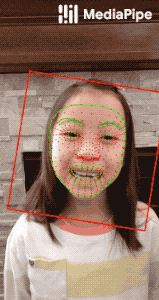
\includegraphics[height=0.3\textwidth,keepaspectratio]{gambar/contoh-mediapipe-face-mesh.png}
  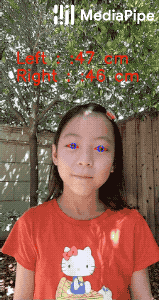
\includegraphics[height=0.3\textwidth,keepaspectratio]{gambar/contoh-mediapipe-iris.png}
  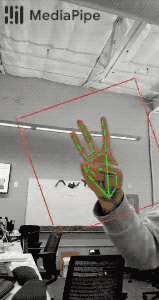
\includegraphics[height=0.3\textwidth,keepaspectratio]{gambar/contoh-mediapipe-hands.png}
  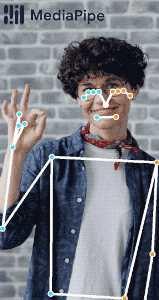
\includegraphics[height=0.3\textwidth,keepaspectratio]{gambar/contoh-mediapipe-pose.png}
  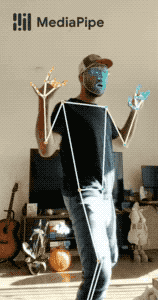
\includegraphics[height=0.3\textwidth,keepaspectratio]{gambar/contoh-mediapipe-holistic.png}
  \caption{Contoh penggunaan MediaPipe untuk deteksi \emph{face mesh}, \emph{iris}, tangan, pose tubuh, dan \emph{holistic} \citep{url:mediapipe}.}
  \label{fig:contohmediapipe}
\end{figure}

MediaPipe merupakan sebuah \emph{machine learning solutions} untuk media \emph{live} dan \emph{streaming}.
MediaPipe memiliki fitur \emph{end-to-end acceleration} yang memungkinkan pemrosesan secara cepat pada perangkat dengan spesifikasi standar serta dapat di-\emph{build} sekali dan di-\emph{deploy} pada berbagai macam \emph{platform} seperti Android, iOS, \emph{desktop}, web, hingga IoT.
MediaPipe merupakan \emph{framework} bersifat \emph{open source},
  menggunakan lisensi Apache 2.0, sehingga dapat dengan mudah dikembangkan sesuai dengan kebutuhan.

Framework ini dapat digunakan pada berbagai macam \emph{platform} dan bahasa pemrograman,
  mulai dari Android, iOS, C++, Python, hingga JavaScript.
Seperti yang terlihat pada gambar \ref{fig:contohmediapipe},
  \emph{framework} ini dapat digunakan untuk melakukan berbagai macam hal mulai dari deteksi wajah, \emph{face mesh}, \emph{iris}, tangan, pose tubuh, \emph{holistic}, dan lain sebagainya.

\subimport{8-mediapipe}{1-mediapipe-pose.tex}
